\section{Financial reasoning becomes a sequence of actions}
\label{sec:execution}

\subsection{Meeting cash shortfalls}

A debt can require several actions even when the debtor owns enough assets. Our census finds 188 episodes entering liquidation, not just the sixty that end the player's game. In 128 episodes the agent raises funds and pays, executing 180 mortgages and eighty-nine building-sale actions. These payments total \$51,997. Sixty-seven take one action, while sixty-one require two to ten. All four systems execute payments: Sol thirty, Gemini thirty-seven, Opus forty-one and Grok twenty (Table~\ref{tab:liquidation}). The counts describe the obligations each encountered and are not comparable difficulty-adjusted success rates.

\begin{table}[t]\centering\small
\begin{tabular}{@{}lrrrr@{}}\toprule
System & Episodes & Paid & Bankruptcy & Paid with building sales\\\midrule
Sol&42&30&12&17\\
Gemini&50&37&13&21\\
Opus&58&41&17&17\\
Grok&38&20&18&13\\\midrule
All&188&128&60&68\\\bottomrule
\end{tabular}
\caption{Every episode requiring an explicit liquidation menu. A sale action can sell multiple buildings; episodes in the last column can also include mortgages. This includes all sixty eliminations but excludes automatic payments from sufficient cash. No new game or branch is executed to count these paths.}
\label{tab:liquidation}\end{table}

The payable obligations provide direct evidence of financial execution. In G20 d327--336, Sol starts with \$49 against \$1,400 and combines \$700 building salvage with \$665 mortgages, paying with \$14 left. More broadly, all 128 payments have sufficient initial own-asset bounds, and the actual event sequence demonstrates the financing used. These are solved local problems with checkable endpoints. They do not establish that the earlier investments that created the shortfall were wise.

Most terminal debts are different: fifty-six exceed even the generous own-asset bound. Of the other four, historical checks find three legal payment sequences. The remaining case, G7 Opus, owes \$750 with nominal resources of \$1,310 but can reach only \$440 through its offered menu. Its hotel cannot be downgraded with zero bank houses, and the menu offers no building sale. Appendix~\ref{app:rules} explains the distinction between this menu and broader bundled-sale validation. Thus the full census separates 128 executed payments, fifty-six insufficient-asset endpoints, one menu restriction and three payable declarations. This is more informative about local competence than a count of bankruptcies alone.

\begin{figure}[t]\centering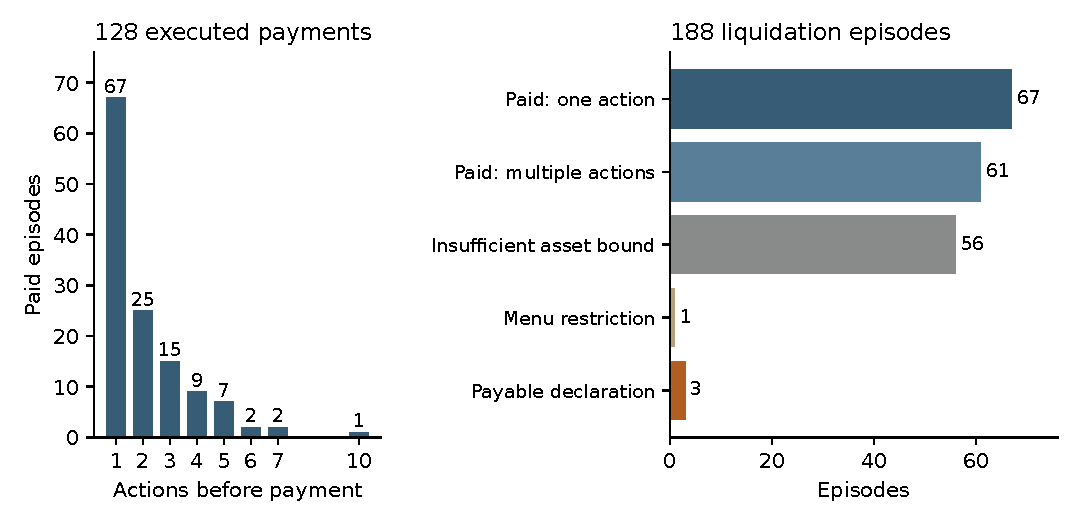
\includegraphics[width=\linewidth]{liquidation_paths.pdf}
\caption{Observed routes through the 188 cash-shortfall episodes. The left panel gives the number of actions in each successful payment; the right separates payment from terminal financing conditions. The fifty-six insufficient-asset classifications use a generous bound, while the three payable declarations use inherited legal-payment checks.}
\label{fig:payments}\end{figure}

\TranscriptTitle{g12}{A payment route is recognized but not executed}
Grok owes \$250 with \$43 cash and seven pink houses. Its private note derives a route through five house sales:
\TranscriptQuote{g12_d249_private_final}
The sole received tool call instead declares bankruptcy:
\TranscriptQuote{g12_d249_public_bankruptcy}
\TranscriptFinding{No sale occurs and the estate transfers to Opus. The historical five-sale sequence pays and leaves \$43. Assistant content requests a two-house sale, which is legal but would reach only \$143, short of the debt.}
\TranscriptReading{The response contains useful multi-step financial reasoning alongside incompatible execution. This is an exception to the many executed payments, and it shows why correctness of one explanation is insufficient to characterize the agent's completed action.}
\TranscriptSource{G12 d249, standard attempt 0. The legal sequence is inherited from the earlier audit, not rerun in this revision.}

\subsection{Financing investment after agreement}

Trade completes sixty-three color groups. All reach a first management window, and forty-three receive construction in that window: Sol 16/17, Gemini 17/18, Opus 7/15 and Grok 3/13. The remaining twenty comprise nine groups with no construction option for that group on any recorded menu in the window, four defaults, four content/call conflicts, and three other valid ends. Availability can itself depend on financing decisions. Seven of the nine receive a mortgaged completing deed; in two cases cash alone can cover redemption and one house, and in five more a static budget including other mortgageable deeds suffices. Those budgets are arithmetic descriptions, not newly executed plans.

Grok's four no-option windows contain stated decisions to defer redemption or development and retain liquidity. Its other six unbuilt windows contain four conflicting calls and two stated holds. Opus's eight comprise five no-option windows under recovery and three defaults. Thus the observed variation combines acquisition terms, financing priorities and execution. A low build fraction cannot simply be read as a preference for cash, nor can every unbuilt group be assigned to the response system.

Historical checks of sixty-one Opus construction defaults preserve the submitted purchase multiset and execute it after splitting count-valued entries and interleaving purchases evenly. The original plans remain invalid. Sixty follow a refused first attempt and invalid recovery; one follows invalid construction and then refusal. This identifies how a feasible investment target can fail at serialization and exhaust its opportunity for correction. It does not establish how a fresh retry would have answered. Other systems do correct many invalid plans: among uneven-build rejections ending in a build, the initial multiset is retained in 20/25 Sol, 6/18 Gemini and 5/5 Grok cases. Changed allocations can also be successful repairs.

The financial scale of subsequent development is substantial, but its interpretation requires exposure. Trade-completed groups receive \$57,378 before loss or game end, of which \$53,810 goes to the forty-three built in their first window. A new descriptive exposure check finds similar median remaining durations, sixty-two versus 63.5 global turns, and forty-two versus forty-seven opponent movements, for first-window-built and other groups. Median receipts are \$590 and \$56. Simple duration alone therefore does not describe the separation, but exact landing opportunities, group type, development levels and selection still differ. Eleven of the twenty other groups build later. These are realized receipts, not incremental returns or an estimated benefit of accelerating construction.

\TranscriptTitle{g20}{A rival's financing becomes the object of a public appeal}
Opus sells Illinois to Grok for \$500, completing reds and leaving Grok \$222. Gemini addresses the table:
\TranscriptQuote{g20-coordination-appeal}
Grok's next note recognizes the appeal. After later construction, it offers Vermont to Gemini for \$150. Gemini refuses:
\TranscriptQuote{g20-concrete-refusal}
\TranscriptFinding{Grok mortgages Vermont for \$50 instead. Opus later offers cash for Grok's property, but neither offer settles. Gemini wins.}
\TranscriptReading{The exchange illustrates a financing externality: buying an otherwise useful deed can supply the rival's construction capital. Gemini calls for financial denial and follows through itself. Opus's later offers show that the table did not uniformly adopt the appeal; the evidence is an attempted coordination with unilateral follow-through, not a functioning cartel.}
\TranscriptSource{G20 d95--102, d129--130 and d156--160. The appeal appears in Grok's d97 request; that decision's content requests a mortgage while its call ends management.}

\subsection{Targets across turns}

The corpus also contains extended targets. In G9, Sol's turn-29 note proposes three houses on each dark-blue deed as funds arrive; financing and construction reach that target on turn 60. G14 d145--148 realizes an initial eight-house target over several management decisions despite changing the first attempted allocation. These cases demonstrate expressed goals with later action, not a measured causal benefit of private memory.

A separate 240-decision, single-reader sample contains fifty-nine prospective own-action statements and thirty-six opponent-oriented statements, with overlap. Eight name a property to buy if landed on; six never encounter that opportunity, one is carried out and one ends in a conflicting purchase/auction response. Fifty-three of sixty Opus sample records lack private notes. We use these records to identify forms of contingent planning, rather than estimate a general completion rate from opportunities that mostly never arise. Likewise, repeated construction errors occur under unequal feedback conditions. They show repair and recurrence, but cannot establish learning or adaptation to unfamiliar opponents.
